% RoTino: modelling and control of a wheeled bipedal robot
% Field and Service Robotics, final technical project, a.y. 2025/2026
%
% Build (from this directory):   pdflatex RoTino_FSR_report && pdflatex RoTino_FSR_report
\documentclass[11pt,a4paper]{article}

\usepackage[utf8]{inputenc}
\usepackage[english]{babel}
\usepackage[a4paper,margin=2.3cm]{geometry}
\usepackage{amsmath,amssymb}
\usepackage{graphicx}
\usepackage{booktabs}
\usepackage{tabularx}
\usepackage{enumitem}
\usepackage{xcolor}
\usepackage[font=small,labelfont=bf,skip=5pt]{caption}
\usepackage{tikz}
\usetikzlibrary{arrows.meta,positioning,calc}
\usepackage[colorlinks=true,linkcolor=black,citecolor=black,urlcolor=black]{hyperref}

\graphicspath{{figures/}}
\setlength{\parskip}{0.35em}
\setlength{\parindent}{1.2em}
\setlist{itemsep=1pt,topsep=3pt,parsep=1pt,leftmargin=1.5em}
\setlist[itemize]{label=$\bullet$}
\setlength{\textfloatsep}{10pt plus 2pt minus 2pt}
\setlength{\floatsep}{8pt plus 2pt minus 2pt}
\setlength{\intextsep}{8pt plus 2pt minus 2pt}
\renewcommand{\topfraction}{0.9}
\renewcommand{\bottomfraction}{0.8}
\renewcommand{\textfraction}{0.08}
\renewcommand{\floatpagefraction}{0.8}

\newcommand{\unit}[1]{\,\mathrm{#1}}
\newcommand{\tc}{\tau_c}
\newcommand{\td}{\tau_d}

\tikzset{
  blk/.style={draw=black!70, fill=black!5, rounded corners=2pt, align=center, font=\footnotesize,
              inner sep=3.5pt, minimum height=9mm},
  key/.style={blk, fill=black!14},
  sig/.style={-{Latex[length=1.7mm]}, semithick, draw=black!80},
  lab/.style={font=\scriptsize, align=center, inner sep=1.5pt},
}

\title{\vspace{-1.2cm}\textbf{RoTino: Modelling and Control of a Wheeled Bipedal Robot}\\[4pt]
\large A cascaded PID built around the Zero Moment Point\\ versus a decoupled MPC + TV-LQR architecture}
\author{Alessandro Prisco \and Aldo Rosicarelli}
\date{\small Field and Service Robotics --- Final technical project, a.y.\ 2025/2026\\
University of Naples Federico II --- October 2026}

\begin{document}
\maketitle
\vspace{-0.6cm}

\begin{abstract}
\noindent RoTino is a 4.3\,kg wheeled bipedal robot: two articulated legs, each ending in a driven wheel, carry a
torso that must be kept in balance like an inverted pendulum. The robot is simulated in Gazebo with
torque control on its six joints. This report describes how it was modelled and how two control laws of very
different nature were designed, implemented and compared on it. The first is a cascaded PID in which the Zero
Moment Point is the variable that the wheels control: a capture-point loop decides where the contact should be
with respect to the centre of mass, and a preview of the planned path makes the robot lean before it accelerates.
The second re-implements the decoupled architecture of Cui \emph{et al.}: a model predictive controller plans the
motion of the upper body, a gain-scheduled LQR balances the wheels and virtual model control drives the legs.
The two laws are run on the same robot, world and scenarios---pushes, constant forces, reference tracking, curved
paths and uneven ground---and the differences in the results are traced back to the design choices that
cause them.
\end{abstract}

% =====================================================================================================
\section{Introduction}

Wheels are fast and efficient on flat ground; legs adapt to obstacles and let a robot change the height and the
attitude of its body. A wheeled bipedal robot puts a driven wheel at the end of each leg and tries to have both
\cite{cui2022,klemm2019}. The price is balance. The robot touches the ground only along the line that joins the two
wheels, so it is an inverted pendulum that has to be stabilised at every instant, and it has fewer actuators than
degrees of freedom.

This is what makes the platform attractive for this course. A single small robot lies at the crossing of the
chapter on wheeled robots and of the chapter on legged robots: its wheels roll without slipping, so its motion on
the plane obeys nonholonomic constraints; its torso is a floating base that can only be moved through the forces
exchanged with the ground; its support polygon degenerates into a segment, so the Zero Moment Point (ZMP) takes a
special role; and it is underactuated, so translation can only be obtained by tilting, much as a quadrotor does.
Although two wheels give the planar motion of a differential drive, the project is not about its kinematic control:
the kinematic layer reduces to a simple heading guidance, and the whole difficulty lies in the underactuated dynamics
of balance.

The robot, named RoTino, is simulated in Gazebo. Two control laws were developed for
it. The first is a cascade of PID loops that was redesigned around the ZMP. The second follows the paper that
guided the project, \emph{Modeling and Control of a Wheeled Biped Robot} by Cui \emph{et al.}~\cite{cui2022}: the
robot is decoupled into a wheeled inverted pendulum of variable length, balanced by a time-varying LQR (TV-LQR),
and a lumped-mass upper body, moved by a model predictive controller (MPC) through virtual model control of the
legs. Having both on the same plant allows a question to be asked that neither answers alone: what does the
model-based, optimisation-based architecture buy with respect to a well-designed cascade, and what does it cost?

\paragraph{Starting point and novelty.} The mechanical model of the robot was available from an earlier simulation,
together with a balance controller that commanded the legs through position servos. Once every joint was
torque controlled and all the loops were closed at 500\,Hz, that controller did not survive the change: the legs
entered a limit cycle. Everything else described in this report was developed in the project:

\begin{itemize}
  \item the modelling of the robot: configuration space and constraints, a planar Lagrangian model, and the two
        reduced models used for control with the parameters of RoTino (Section~\ref{sec:model});
  \item a cascaded PID controller designed around the ZMP and the capture point, with a preview of the planned path
        and a gain design supported by a robustness analysis (Section~\ref{sec:pid});
  \item an implementation of the architecture of Cui \emph{et al.}\ on RoTino (Section~\ref{sec:mpc});
  \item a benchmark of eleven scenarios run with both laws, in which the ZMP is reconstructed from the multibody
        dynamics because the simulator does not provide contact forces (Section~\ref{sec:results}).
\end{itemize}

The two authors worked jointly on every part of the project---modelling, both controllers, the benchmark and the
analysis of the results---so no separate attribution of the work is made.

% =====================================================================================================
\section{The robot}
\label{sec:model}

\subsection{RoTino}

RoTino (Fig.~\ref{fig:robot}a) has a box-shaped torso and two identical legs. Each leg is a planar chain of a
thigh and a shank of equal length, with a hip and a knee joint whose axes are parallel to the wheel axle, and ends
in a driven wheel. All six joints are torque controlled. In the nominal posture thigh and shank are at
$\pm 45^\circ$, so the wheel axle sits exactly below the hips. Table~\ref{tab:params} lists the parameters that
matter for control.

Two features of this small robot shape the control problem. First, about four fifths of the mass sit above the
wheels and close to them: the equivalent pendulum is only 16\,cm long, which makes the unstable dynamics fast.
Second, the centre of mass (CoM) of the upper body is not above the hips but about one centimetre ahead of them.
With the wheels under the hips the equivalent pendulum already leans by almost $5^\circ$: a controller cannot assume
that ``torso upright'' means ``balanced'', and has to find the equilibrium by itself.

\begin{figure}[t]
  \centering
  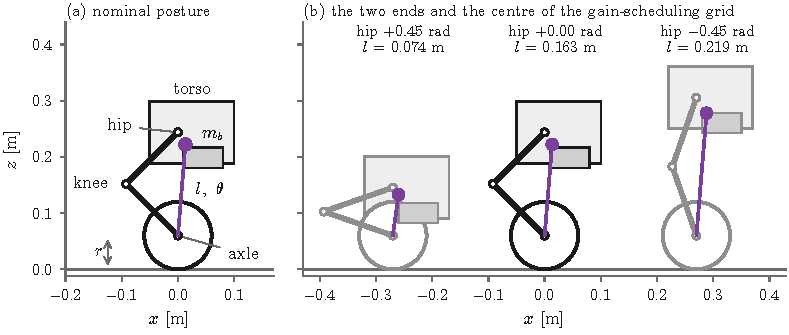
\includegraphics[width=\linewidth]{fig_robot.pdf}
  \caption{Sagittal view of RoTino, drawn to scale. The purple segment is the equivalent pendulum
  used for control: it joins the wheel axle to the centre of mass $m_b$ of everything above the wheels, with length
  $l$ and lean angle $\theta$ from the vertical. Folding or stretching the legs changes $l$ by a factor of three.}
  \label{fig:robot}
\end{figure}

\begin{table}[t]
  \centering\small
  \caption{Main parameters of RoTino (rounded).}
  \label{tab:params}
  \begin{tabular}{@{}llr@{\hspace{10mm}}llr@{}}
    \toprule
    total mass & $M$ & 4.3\,kg & thigh and shank length & $l_1=l_2$ & 0.13\,m \\
    mass above the wheels & $m_b$ & 3.5\,kg & wheel radius & $r$ & 0.06\,m \\
    mass of one wheel & $m_w$ & 0.38\,kg & distance between the wheels & $d$ & 0.29\,m \\
    pendulum length (nominal) & $l$ & 0.16\,m & hip height (nominal) & & 0.24\,m \\
    CoM height (nominal) & $h$ & 0.19\,m & wheel--ground friction & $\mu$ & 2.2 \\
    wheel torque used & & $\pm 10$\,Nm & leg torque used & & $\pm 50$\,Nm \\
    \bottomrule
  \end{tabular}
\end{table}





\subsection{Configuration space, constraints and underactuation}

Before any contact is imposed, the robot is a floating base with six joints. The torso is a rigid body in space
with six degrees of freedom (DoF), and each of the two hips, two knees and two wheels adds one: twelve in total.
The shape of the configuration space follows from the nature of each coordinate. The pose of the torso lives in
$SE(3)$; hips and knees have mechanical limits, so each spans a closed interval rather than a circle; the wheels
turn indefinitely, so together they span a torus. The configuration space is therefore
$SE(3)\times I^4\times T^2$, where $I$ is an interval. The orientation of the torso is described with quaternions,
an implicit representation that avoids the singularities of a three-angle parameterisation.

Contact with the ground adds constraints of two kinds, and the distinction matters because only one of them reduces
the configuration space. With both wheels on flat ground, the height and the roll of the torso are no longer free:
they follow from the pitch and from the leg joints. These constraints are \emph{holonomic}. Rolling without slipping
is different. The two wheels impose that the axle midpoint cannot move sideways and that its forward speed $\dot s$
and the yaw rate $\dot\varphi$ are tied to the wheel speeds $\omega_l,\omega_r$:
\begin{equation}
  \dot x\sin\varphi-\dot y\cos\varphi=0,\qquad
  \dot s=\tfrac{r}{2}(\omega_l+\omega_r),\qquad \dot\varphi=\tfrac{r}{d}(\omega_r-\omega_l).
  \label{eq:rolling}
\end{equation}
The first relation is not integrable: it restricts the velocities, not the positions that can be reached, and
is a \emph{nonholonomic} constraint in Pfaffian form. On the plane RoTino therefore moves like a differential
drive. Two consequences are used later: the position of the robot can be reconstructed by integrating
\eqref{eq:rolling} (the odometry of Section~\ref{sec:estimator}), and a lateral error can be corrected only while
moving (the guidance of Section~\ref{sec:heading}).

Underactuation, as stressed in the course, is a property of the model used to describe the robot rather than of the
robot itself, so it is worth counting it at the three levels at which RoTino is modelled (Table~\ref{tab:under}). At
every level exactly one degree of freedom has no actuator, and it is always the same one: the pitch of the body
about the wheel axle. No motor acts between the body and the ground. A wheel motor pushes the wheel forward and,
by reaction, the body backward; this inertial coupling is the only handle on the pitch.

\begin{table}[t]
  \centering\small
  \caption{Degrees of freedom $n$ and actuators $m$ of the models of RoTino.}
  \label{tab:under}
  \begin{tabular}{@{}lccl@{}}
    \toprule
    Model & $n$ & $m$ & Free coordinates \\
    \midrule
    robot on the ground, rolling & 7 & 6 & forward position, yaw, pitch, four leg joints \\
    sagittal planar model & 4 & 3 & shank, wheel, knee, torso \\
    wheeled pendulum (sagittal) & 2 & 1 & forward position, pitch \\
    \bottomrule
  \end{tabular}
\end{table}

\subsection{Planar Lagrangian model}

When both legs move together the robot reduces to a planar chain: wheel, shank, thigh and torso. With the absolute
angle of the shank $q_1$, the rotation of the wheel $q_w$, the knee angle $q_2$ and the pitch of the torso $q_3$ as
coordinates, the Euler--Lagrange equations take the usual form
\begin{equation}
  M(q)\,\ddot q+C(q,\dot q)\,\dot q+g(q)=B\,\tau,\qquad \tau=(\tau_w,\ \tau_{knee},\ \tau_{hip}).
  \label{eq:lagrange}
\end{equation}
This model was derived symbolically for RoTino; here it is used for what it shows rather than for its expressions.
The matrix $B$ has three columns for four coordinates, and it was built from the virtual work of the motors: each
motor acts between two bodies, so its column is the gradient of the relative angle between them. A simple test
follows from this. A rigid rotation of the whole robot about the axle changes no relative angle, hence no motor
can do work on it: the coordinate associated with that motion---the pitch of the body---is passive. In the language
of partial feedback linearisation~\cite{spong1994}, the pitch can only be controlled through a non-collocated
scheme, by using the actuated coordinates to produce the inertial forces that move the passive one. Both controllers
of this report do exactly this, each in its own way. The planar model also served as an independent check of the
reduced models introduced next: they give the same position of the CoM for the same posture.

\subsection{The reduced models used for control}
\label{sec:reduced}

Neither controller uses \eqref{eq:lagrange} directly. Following Cui \emph{et al.}~\cite{cui2022}, the robot is
split into two simple models, each of which captures one part of the problem.

\paragraph{Equivalent pendulum.} Everything above the wheels---torso, thighs and shanks---is replaced by its
centre of mass. Its position with respect to the axle, computed from the joint angles through the
forward kinematics, defines a pendulum of length $l$ and lean angle $\theta$ (Fig.~\ref{fig:robot}). When the legs
fold or stretch, $l$ changes from 7 to 22\,cm: the pendulum has a \emph{variable length}.

\paragraph{Wheeled inverted pendulum.} The wheels and this pendulum form the variable-length wheeled inverted
pendulum (VL-WIP). Its state collects the forward position $s$ of the axle, the lean $\theta$, the yaw $\varphi$ and
their rates; the inputs are the two wheel torques. Linearised about the upright equilibrium it reads
\begin{equation}
  \ddot s=a_1(l)\,\theta+b_1(l)\,(\tau_l+\tau_r),\qquad
  \ddot\theta=a_2(l)\,\theta+b_2(l)\,(\tau_l+\tau_r),\qquad
  \ddot\varphi=b_3\,(\tau_r-\tau_l),
  \label{eq:vlwip}
\end{equation}
with the coefficients given in closed form in~\cite{cui2022} as functions of the masses, of the wheel inertia and
of $l$. Equation~\eqref{eq:vlwip} already tells most of the story. The sum of the torques drives balance and
forward motion together, their difference drives the yaw alone: it is natural to work with the common torque
$\tc=(\tau_l+\tau_r)/2$ and the differential torque $\td=(\tau_r-\tau_l)/2$. Moreover $a_2>0$ and $b_2<0$: the
lean is unstable, and a forward torque tilts the body backward.

Two numbers summarise the sagittal dynamics of RoTino (Fig.~\ref{fig:lqr}a). The unstable pole is at about
10\,rad/s: left alone, a lean doubles in less than a tenth of a second. The transfer function from the common
torque to the position has a zero in the right half-plane at about 6\,rad/s: the system is \emph{non-minimum
phase}. Physically, to move forward the wheels must first roll backward, so that the body falls forward, and
only then accelerate. Any controller has to respect this order of events; the two controllers of this report differ
precisely in how they plan it.

\paragraph{Lumped-mass upper body.} The second model describes how the CoM moves when it is displaced from the
wheels. Let $\delta$ be the horizontal distance of the CoM ahead of the contact point, $h$ its height and $F_z$ the
vertical force of the legs. If the resultant of gravity and inertia is to pass through the contact, as it must
since the wheel cannot transmit a moment,
\begin{equation}
  \ddot c=\frac{g+\ddot z}{h}\,\delta,\qquad \ddot z=\frac{F_z}{m_b}-g ,
  \label{eq:lumped}
\end{equation}
where $c=s+\delta$ is the horizontal position of the CoM. The first relation is the centrepiece of both
controllers. With $\ddot z=0$ it is the linear inverted pendulum, $\ddot c=\omega^2(c-p)$ with $\omega=\sqrt{g/h}$
and $p$ the position of the contact: the CoM accelerates away from the contact, in proportion to the offset. For
RoTino $\omega\approx 7$\,rad/s. Whoever controls $\delta$ controls the acceleration of the robot; the MPC calls
it $\Delta s$ and optimises it over a horizon, the PID calls it the ZMP offset and regulates it with a cascade.

\begin{figure}[t]
  \centering
  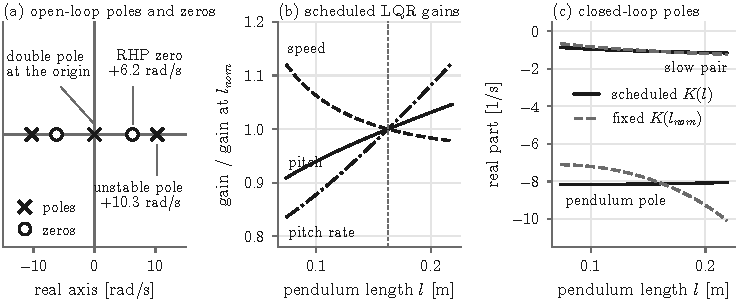
\includegraphics[width=\linewidth]{fig_vlwip_lqr.pdf}
  \caption{(a) Poles and zeros of the linearised pendulum, from the common torque to the position, in the nominal
  posture: one unstable pole and one right-half-plane (RHP) zero. (b) LQR gains of the common torque on speed, pitch
  and pitch rate over the 25 postures of the schedule, relative to their nominal value; the gain on the position
  does not change. (c) Dominant closed-loop poles with the scheduled gain and with the nominal gain kept fixed.}
  \label{fig:lqr}
\end{figure}

% =====================================================================================================
\section{First controller: a cascaded PID built around the ZMP}
\label{sec:pid}

\subsection{The ZMP as the control input}

For a legged robot the ZMP is usually a constraint: the point where the ground reaction produces no horizontal
moment must stay inside the support polygon, and motions are planned so that it does~\cite{vukobratovic2004}. On two
wheels the picture changes. The support polygon is the segment between the two contacts. Sideways the ZMP can
move along it and must remain inside it, as usual. In the direction of travel, however, the segment has no
width: the ZMP necessarily lies on the contact line, and the wheels decide where that line is. The ZMP is no longer
a quantity to be kept within bounds but the natural \emph{input} of the balance: rolling the wheels moves it,
and by \eqref{eq:lumped} the offset $\delta=c-p$ between CoM and ZMP sets the acceleration of the CoM. This is the
cart--table view of Kajita \emph{et al.}~\cite{kajita2003}, read for a robot whose ``table'' is a pair of wheels.

The controller is organised accordingly (Fig.~\ref{fig:pidarch}). An outer loop decides which offset is needed;
an inner loop makes the wheels realise it; the heading uses the differential torque; the legs keep the posture.
All the quantities it needs---the CoM, the contact line, the heading---are computed from the
pose of the torso and the joint angles. In this controller the pose of the torso is taken from the simulator; the
consequences of this choice for the comparison are discussed in Section~\ref{sec:benchmark}.

\begin{figure}[t]
  \centering
  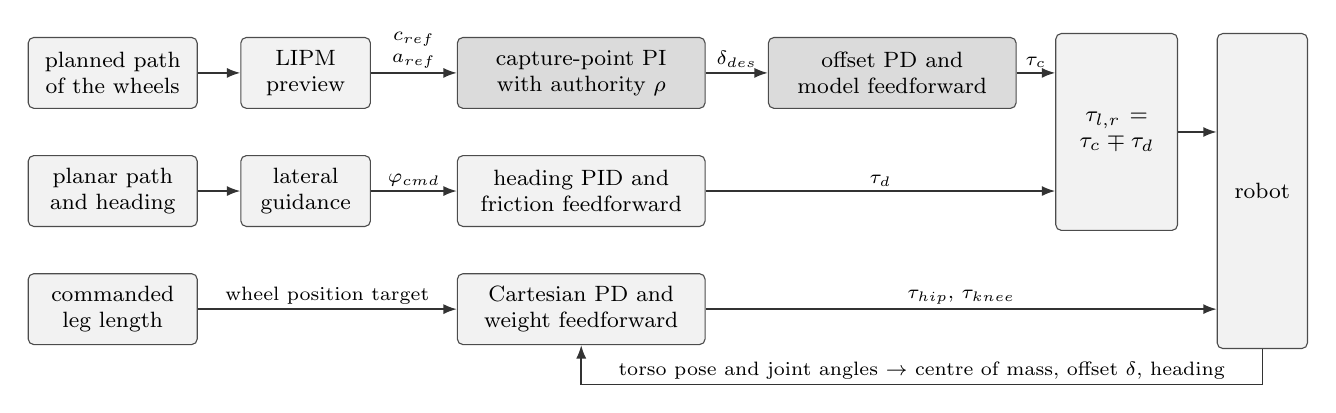
\begin{tikzpicture}
    \node[blk, text width=19mm] (path) at (1.1,0) {planned path\\ of the wheels};
    \node[blk, text width=14mm] (prev) at (3.55,0) {LIPM\\ preview};
    \node[key, text width=29mm] (cp) at (7.05,0) {capture-point PI\\ with authority $\rho$};
    \node[key, text width=29mm] (pd) at (11.0,0) {offset PD and\\ model feedforward};
    \node[blk, text width=19mm] (traj) at (1.1,-1.5) {planar path\\ and heading};
    \node[blk, text width=14mm] (guid) at (3.55,-1.5) {lateral\\ guidance};
    \node[blk, text width=29mm] (yaw) at (7.05,-1.5) {heading PID and\\ friction feedforward};
    \node[blk, text width=19mm] (sup) at (1.1,-3.0) {commanded\\ leg length};
    \node[blk, text width=29mm] (leg) at (7.05,-3.0) {Cartesian PD and\\ weight feedforward};
    \node[blk, text width=13mm, minimum height=25mm] (mix) at (13.85,-0.75) {$\tau_{l,r}=$\\ $\tc\mp\td$};
    \node[blk, text width=9mm, minimum height=40mm] (rob) at (15.7,-1.5) {robot};
    \draw[sig] (path) -- (prev);
    \draw[sig] (prev) -- node[lab, above]{$c_{ref}$\\ $a_{ref}$} (cp);
    \draw[sig] (cp) -- node[lab, above]{$\delta_{des}$} (pd);
    \draw[sig] (pd) -- node[lab, above]{$\tc$} (pd -| mix.west);
    \draw[sig] (traj) -- (guid);
    \draw[sig] (guid) -- node[lab, above]{$\varphi_{cmd}$} (yaw);
    \draw[sig] (yaw) -- node[lab, above, pos=0.5]{$\td$} (yaw -| mix.west);
    \draw[sig] (sup) -- node[lab, above]{wheel position target} (leg);
    \draw[sig] (leg) -- node[lab, above, pos=0.5]{$\tau_{hip}$, $\tau_{knee}$} (leg -| rob.west);
    \draw[sig] (mix) -- (mix -| rob.west);
    \draw[sig] (rob.south) -- ++(0,-0.45) -| node[lab, above, pos=0.25]{torso pose and joint angles $\rightarrow$ centre
      of mass, offset $\delta$, heading} (leg.south);
  \end{tikzpicture}
  \caption{Architecture of the cascaded PID. The two shaded blocks form the sagittal cascade: the outer one decides
  where the contact should be with respect to the centre of mass, the inner one makes the wheels realise it. The
  measurements reach every block; a single feedback path is drawn for clarity.}
  \label{fig:pidarch}
\end{figure}

\subsection{The sagittal cascade}

\paragraph{Outer loop: the capture point.} The linear pendulum has one stable and one unstable mode, and the
unstable one is carried by the \emph{capture point} $\xi=c+\dot c/\omega$, the point where the contact would have
to be for the robot to come to rest~\cite{pratt2006}. Its dynamics is of first order and is driven directly by
the ZMP:
\begin{equation}
  \dot\xi=\omega\,(\xi-p).
  \label{eq:dcm}
\end{equation}
Controlling the capture point therefore controls the only part of the motion that diverges, and it requires nothing
but a choice of $p$~\cite{englsberger2011}. Let $e_c$ be the error of the CoM with respect to its reference and
$e_\xi=e_c+\dot e_c/\omega$ the corresponding error of the capture point. Asking $e_\xi$ to decay at a rate $k_\xi$,
with an integral term to absorb constant disturbances, and solving \eqref{eq:dcm} for the contact gives the offset
that the wheels should produce:
\begin{equation}
  \delta_{des}=\delta_{ff}-\frac{\rho}{\omega}\Big(\dot e_c+k_\xi\,e_\xi+k_I\!\int\! e_\xi\,dt\Big),
  \qquad |\delta_{des}|\le\frac{a_{max}}{\omega^2}.
  \label{eq:outer}
\end{equation}
The term $\delta_{ff}$ is a feedforward, discussed below, and $\rho\in(0,1]$ is the \emph{authority} of the loop,
whose role is the subject of Section~\ref{sec:authority}. The bound limits the acceleration that the controller may
ask for to $a_{max}=3\unit{m/s^2}$; for RoTino this is an offset of about 6\,cm, that is a lean of more than
$20^\circ$. The integral is itself bounded, as an anti-windup measure. Both bounds will be visible in the results.

\paragraph{Inner loop: the offset.} The wheels have to place the contact so that the measured offset $\delta$
follows $\delta_{des}$. A PD on the offset, added to a feedforward torque, gives the common wheel torque:
\begin{equation}
  \tc=\tau_{ff}+K_\delta\,(\delta-\delta_{des})+D_\delta\,(\dot\delta-\dot\delta_{ff}).
  \label{eq:inner}
\end{equation}
The sign is the one that the non-minimum-phase plant requires: if the CoM is too far ahead of the contact, the
wheels are driven forward to catch up with it.

\paragraph{Feedforward from the model.} To hold a constant acceleration $a$ without changing its lean, the
pendulum~\eqref{eq:vlwip} needs a definite lean and a definite torque, obtained by setting $\ddot\theta=0$,
$\ddot s=a$. The solution is proportional to $a$: about 22\,mm of offset and 0.17\,Nm per wheel for each
$\unit{m/s^2}$. The offset is close to the value $h/g$ of the simple pendulum~\eqref{eq:lumped}; the small
difference is the contribution of the wheel inertia, which the VL-WIP model includes. These two constants give
$\delta_{ff}$ and $\tau_{ff}$ from the reference acceleration, so the feedback only has to correct what the model
does not predict.

\subsection{Preview of the planned path}

What reference should the CoM follow when the wheels are asked to follow a path $p_{ref}(t)$? Because of the
right-half-plane zero, it cannot be the path itself: the CoM must already be ahead of the wheels when they start to
accelerate. The reference is the solution of the pendulum equation $\ddot c_{ref}=\omega^2(c_{ref}-p_{ref})$ that
stays bounded, and this solution is not causal: it is the planned path smoothed by a two-sided exponential kernel,
\begin{equation}
  c_{ref}(t)=\frac{\omega}{2}\int_{-\infty}^{+\infty} e^{-\omega|u|}\,p_{ref}(t+u)\,du .
  \label{eq:preview}
\end{equation}
The CoM reference thus looks about $1/\omega\approx0.14$\,s ahead and behind; in
practice the integral is a weighted sum over a window of the planned path. The reference acceleration
$a_{ref}=\omega^2(c_{ref}-p_{ref})$ that enters the feedforward is a smoothed version of the acceleration of the
path that starts \emph{before} it (Fig.~\ref{fig:preview}): the robot begins to lean a few tenths of a second
before the wheels are asked to move. This is the ZMP preview of walking pattern generators~\cite{kajita2003},
applied here to a known path. When the robot is driven by live commands the future is unknown, and the feedforward
falls back on the current, rate-limited acceleration of the command.

\begin{figure}[t]
  \centering
  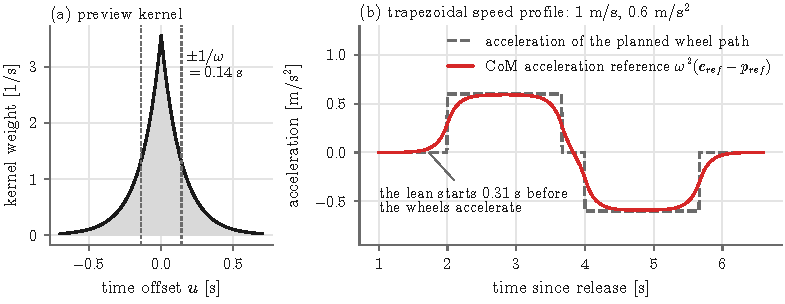
\includegraphics[width=0.72\linewidth]{fig_lipm_preview.pdf}
  \caption{The preview of the planned path for a trapezoidal speed profile (1\,m/s, 0.6\,m/s$^2$): the acceleration
  of the path is a sequence of steps, and the acceleration reference obtained with the preview anticipates each of
  them.}
  \label{fig:preview}
\end{figure}

\subsection{Why the outer loop has reduced authority}
\label{sec:authority}

With $\rho=1$, \eqref{eq:outer} is the textbook capture-point controller. It rests on an assumption: that the
contact can be placed instantly where the outer loop wants it. Here this is not true. The inner loop moves the
contact by accelerating a wheel against a pendulum whose own dynamics is at about 10\,rad/s, the control runs at
500\,Hz, and one or two samples of delay separate a measurement from the torque it produces.

To choose the gains, the cascade \eqref{eq:outer}--\eqref{eq:inner} was closed on the linear model
\eqref{eq:vlwip}, sampled at 500\,Hz with one and two samples of delay, for ten cases: the nominal robot, an upper
body 20\,\% lighter and heavier, and the legs folded and stretched. Figure~\ref{fig:authority} summarises what this
analysis shows. With full authority the dominant poles include an oscillatory pair, and the inner stiffness
$K_\delta$ can be less than doubled before some of the ten cases become unstable. Reducing the authority brings
those poles back to the real axis and widens the stable range of $K_\delta$. The value $\rho=0.4$ is where the
dominant poles are best damped; the stiffness chosen for the inner loop, 60\,Nm per metre of offset, then has a
margin of about four. The price is that the outer loop corrects a position error more slowly, and the integral term
is there to recover what the reduced authority leaves. The same linear model was used to
check the control law before simulating the robot: tracking of the trapezoid, rejection of the push of the benchmark
and removal of an unknown offset of the CoM.

\begin{figure}[t]
  \centering
  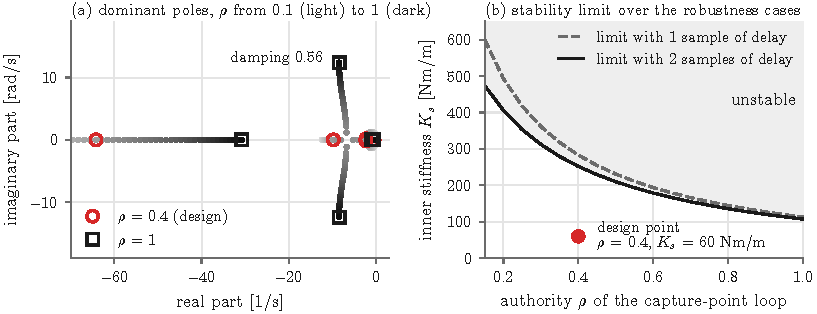
\includegraphics[width=\linewidth]{fig_pid_authority.pdf}
  \caption{Choice of the authority $\rho$ of the capture-point loop on the sampled linear model. (a) With full
  authority an oscillatory pair appears; with $\rho=0.4$ the dominant poles are real. (b) Largest inner stiffness
  for which all the robustness cases remain stable: the lower the authority, the wider the margin.}
  \label{fig:authority}
\end{figure}

\subsection{Heading and lateral guidance}
\label{sec:heading}

The yaw equation in \eqref{eq:vlwip} is a double integrator driven by the differential torque, so a PID on the
heading error is adequate, with one addition. When the robot turns, its wide wheels scrub on the ground. Without
compensation the yaw advances in jerks (stick--slip), and the lateral dynamics of the robot no longer follows the
planned turn. A feedforward, computed from the \emph{reference} yaw rate so that it cannot chatter, supplies the
Coulomb and viscous friction torque identified in simulation.

To follow a path on the plane, the heading reference is corrected by the lateral error $e_y$ of the axle with
respect to the path:
\begin{equation}
  \varphi_{cmd}=\varphi_{ref}-\arctan(k_y\,e_y)\cdot\min\!\big(1,\ |v_{ref}|/v_0\big).
  \label{eq:guidance}
\end{equation}
The robot steers towards the path by an angle that grows with the error and saturates, and the correction fades
out as the reference speed goes to zero. The last factor is the practical face of the nonholonomic
constraint~\eqref{eq:rolling}: a differential drive cannot move sideways, so a lateral error can only be removed
while travelling, and a smooth time-invariant feedback cannot regulate the full pose at
standstill~\cite{brockett1983}. The path itself is planned as in the course, with a geometric path and a separate
timing law: the S-curve is a cubic polynomial $y(x)$ that leaves and arrives parallel to the initial heading,
travelled with a quintic law in the arc length.

The common and the differential torque are finally mixed as $\tau_{l,r}=\tc\mp\td$. When the sum would exceed the
torque limit, it is the common torque that keeps priority: a robot that turns late is a nuisance, one that falls
is a failure.

\subsection{Legs}

In this controller the legs are a positioning device: they hold the wheel under the hip at the commanded leg
length. Each leg has a Cartesian PD on the position $p$ of the wheel centre with respect to the hip, with the
share of the weight it carries as feedforward, mapped to joint torques by the transpose of the leg Jacobian $J$:
\begin{equation}
  \tau_{leg}=J^{T}\big(K_p\,(p_d-p)-K_d\,\dot p+F_{ff}\big).
  \label{eq:legs}
\end{equation}
Working in Cartesian space was the remedy for the limit cycle mentioned in the introduction. The joint-space gains
inherited from the position-servo controller were so high that, at 500\,Hz, a single control step could reverse the
velocity of the light leg links; the Cartesian gains correspond to a joint stiffness about three times lower, and
the oscillation disappears.

A compensation of the \emph{lateral} ZMP was also implemented: in a turn the legs are made unequal in length so
that the torso leans into the curve, as a cyclist does, with the same preview as in the sagittal plane. It is
disabled by default, because with the rigid cylindrical wheels of the model the lean moves the contact onto the
wheel edge and disturbs the yaw; the results below show that the lateral margin is in any case large.

% =====================================================================================================
\section{Second controller: MPC, TV-LQR and virtual model control}
\label{sec:mpc}

\subsection{The architecture of the paper and its implementation}

Cui \emph{et al.}~\cite{cui2022} place their method between two extremes: controllers that treat the robot as a
plain wheeled pendulum and ignore the legs and the torso, and whole-body controllers, which are complete but
complex. Their proposal assigns each of the two models of Section~\ref{sec:reduced} to the controller that suits
it. Balance is fast and unstable, but it is well described by a linear model, so it is given to an LQR on the
wheels. The motion of the upper body is slower, but it is subject to limits---friction, leg length, available
force---so it is given to an MPC, which can handle constraints. The MPC does not command torques: it decides the
offset $\delta$ of the CoM and the vertical force $F_z$, and virtual model control turns them into leg torques.
A Kalman filter provides the state. Figure~\ref{fig:mpcarch} shows the resulting architecture.

Unlike the PID of the previous section, this controller uses only the sensors that a real robot would carry: the
IMU and the joint encoders. The true pose given by the simulator is used only to evaluate the estimation error.

\begin{figure}[t]
  \centering
  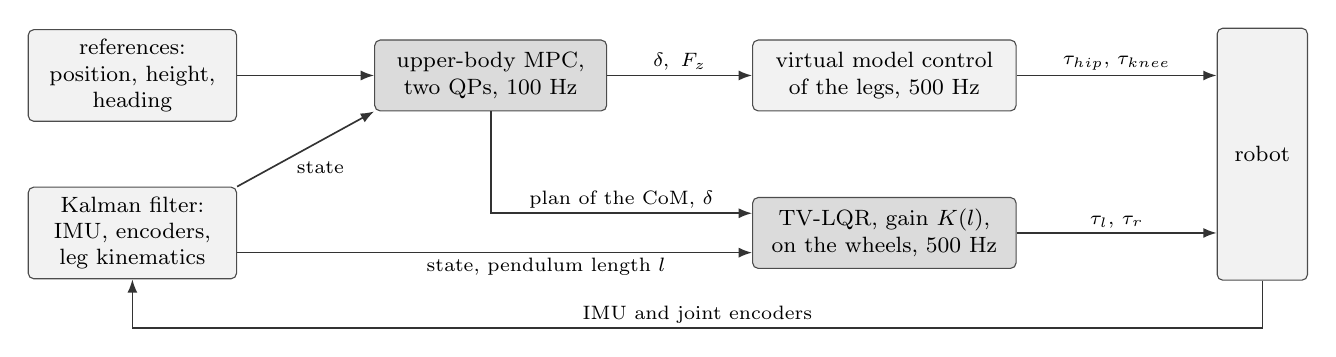
\begin{tikzpicture}
    \node[blk, text width=24mm] (ref) at (1.35,0) {references:\\ position, height,\\ heading};
    \node[blk, text width=24mm] (est) at (1.35,-2.0) {Kalman filter:\\ IMU, encoders,\\ leg kinematics};
    \node[key, text width=27mm] (mpc) at (5.9,0) {upper-body MPC,\\ two QPs, 100 Hz};
    \node[blk, text width=31mm] (vmc) at (10.9,0) {virtual model control\\ of the legs, 500 Hz};
    \node[key, text width=31mm] (lqr) at (10.9,-2.0) {TV-LQR, gain $K(l)$,\\ on the wheels, 500 Hz};
    \node[blk, text width=9mm, minimum height=32mm] (rob) at (15.7,-1.0) {robot};
    \draw[sig] (ref) -- (mpc);
    \draw[sig] (mpc) -- node[lab, above]{$\delta,\ F_z$} (vmc);
    \draw[sig] (mpc.south) |- node[lab, above, pos=0.75]{plan of the CoM, $\delta$} ([yshift=2.5mm]lqr.west);
    \draw[sig] (vmc) -- node[lab, above]{$\tau_{hip}$, $\tau_{knee}$} (vmc -| rob.west);
    \draw[sig] (lqr) -- node[lab, above]{$\tau_l$, $\tau_r$} (lqr -| rob.west);
    \draw[sig] (est.north east) -- node[lab, below right, pos=0.4]{state} (mpc.south west);
    \draw[sig] ([yshift=-2.5mm]est.east) -- node[lab, below, pos=0.6]{state, pendulum length $l$} ([yshift=-2.5mm]lqr.west);
    \draw[sig] (rob.south) -- ++(0,-0.6) -| node[lab, above, pos=0.25]{IMU and joint encoders} (est.south);
  \end{tikzpicture}
  \caption{Architecture of the second controller. The MPC plans the motion of the upper body; the LQR, whose gain
  follows the length of the pendulum, makes the wheels follow that plan; virtual model control realises the planned
  offset and vertical force with the legs.}
  \label{fig:mpcarch}
\end{figure}

\subsection{State estimation}
\label{sec:estimator}

The estimator answers the question that the PID avoided: where is the torso, and how fast is it moving, if the
only data are those of the robot itself? Two sources are available, with opposite defects. The accelerations of
the IMU, rotated to the world frame and integrated, are accurate over short times but drift. The wheels, through
the rolling constraint~\eqref{eq:rolling} and the kinematics of the legs, give the position and the velocity of the
torso without drift, but they are wrong whenever a wheel slips or leaves the ground. As in the paper, a linear
Kalman filter merges them. For each axis the state is the position and the velocity of the torso; the prediction
integrates the measured acceleration $a$ over the sampling time $T$, and the correction compares the result with the
position and velocity obtained from odometry:
\begin{equation}
  \begin{bmatrix} p\\ v\end{bmatrix}_{k+1}=
  \begin{bmatrix} 1&T\\0&1\end{bmatrix}\begin{bmatrix} p\\ v\end{bmatrix}_{k}
  +\begin{bmatrix}T^2/2\\ T\end{bmatrix}a_k,
  \qquad
  y_k=\begin{bmatrix}p_{axle}+p_{torso/axle}\\ v_{axle}+v_{torso/axle}\end{bmatrix}.
  \label{eq:kalman}
\end{equation}
At steady state the filter behaves as a complementary filter: odometry prevails at low frequency, the IMU above a
few hertz. Because the three axes are decoupled, three independent two-state filters are used, which
is equivalent and cheaper. If the wheels lose contact with the ground they carry no information, and the correction
is simply skipped. The lean $\theta$ and the
length $l$ of the pendulum do not need a filter: they follow from the orientation given by the IMU and from the
leg kinematics.

\subsection{Balance: a gain-scheduled LQR}

The wheels are driven by a state feedback on the model \eqref{eq:vlwip}. With $\tilde x$ the error of the state
$x=(s,\theta,\varphi,\dot s,\dot\theta,\dot\varphi)$ with respect to its reference and $u=(\tau_l,\tau_r)$, the gain
minimises
\begin{equation}
  J=\int_0^\infty\big(\tilde x^{T}Q\,\tilde x+u^{T}R\,u\big)\,dt,\qquad u=-K(l)\,\tilde x .
  \label{eq:lqr}
\end{equation}
The model depends on the length of the pendulum, hence so does the gain: this is what the paper calls a
time-varying LQR. Here the Riccati equation is solved once, in advance, for 25 leg postures
between a deep squat and full extension, and the gain is interpolated on the current value of $l$. The solution
is obtained from the stable invariant subspace of the Hamiltonian matrix of the problem.

Three aspects of the design deserve a comment.

\emph{The weights.} $Q$ penalises the lean far more than the position, so that balance has priority over
tracking. $R$ is not chosen in the coordinates of the two motors but in those of the common and of the
differential torque, with the differential one weighted fifty times more. The reason came from simulation: the
torso, held by the virtual springs of the legs, has a torsional resonance at about 12\,Hz, and a stiff yaw loop
excites it into a sustained oscillation. The heavy weight keeps the yaw loop slow and well below that frequency.
The cost of this choice appears in the results on curved paths.

\emph{The effect of scheduling.} Figure~\ref{fig:lqr}b--c shows what the schedule does on a robot of this size.
Over the whole range of leg lengths the gains change by about 15\,\%, and they keep the dominant closed-loop poles
almost exactly where they were designed. With the nominal gain kept fixed the loop remains stable, but its poles
move with the posture. For RoTino scheduling is therefore a refinement that makes the response independent of the
height.

\emph{The reference.} The LQR is not asked to follow the trajectory requested by the operator. Its reference is
built from the output of the MPC,
\begin{equation}
  x_{ref}=\big(c_{plan}-\delta,\ \ \arctan(\delta/z_{ref}),\ \ \varphi_{cmd},\ \ \dot c_{plan},\ \ 0,\ \ \dot\varphi_{ref}\big):
  \label{eq:xref}
\end{equation}
the lean is the one that corresponds to the planned offset at the reference height $z_{ref}$, and the position and
the speed are those that the MPC predicts for the CoM in the next instants, the position being shifted back by
$\delta$ because the wheels must stay behind a CoM that leans forward. The LQR thus tracks a plan that already
respects the limits of the robot, and it never receives a reference that it could follow only by violating them. The friction feedforward
and the slow integral on the heading described in Section~\ref{sec:heading} are added to the differential torque
here as well.

\subsection{Upper body: a constrained MPC}

The MPC works on the lumped-mass model~\eqref{eq:lumped}. Over a horizon of 25 steps of 20\,ms, half a second in
all, it chooses the sequences of the offset $\delta$ and of the vertical force $F_z$ that minimise the deviation of
the CoM from its reference and the control effort,
\begin{equation}
  \min\ \sum_{i=1}^{N}\Big[(x_i-x_i^{ref})^{T}S\,(x_i-x_i^{ref})+w\,u_i^2\Big]
  \qquad\text{subject to}\quad |\delta|\le\delta_{max},\quad F_{min}\le F_z\le F_{max},
  \label{eq:mpc}
\end{equation}
and applies the first element of each sequence. It runs at 100\,Hz, once every five control steps.

\paragraph{Two small problems instead of one.} Over the horizon the factor $(g+\ddot z)/h$ of \eqref{eq:lumped} is
frozen at its current value. The horizontal and the vertical dynamics then become two independent double
integrators, one driven by $\delta$ and one by $F_z$, and \eqref{eq:mpc} splits into two problems with a single
input each. Each double integrator is discretised exactly over the step of 20\,ms.

\paragraph{The constraints.} The offset is bounded by $\delta_{max}=3$\,cm, which corresponds to a lean of about
$10^\circ$: whatever happens, the plan never asks the robot to lean more than that. The
vertical force is bounded between a fraction and a multiple of the weight of the upper body, so that the wheels
neither lift off nor are pressed beyond what the legs can deliver.

\paragraph{Solving the problem.} Eliminating the states (\emph{condensing}~\cite{jerez2011}) leaves a quadratic
program in the 25 inputs alone, whose only constraints are bounds on the variables. A problem of this kind does
not need a general solver: the projection onto the bounds is a simple clipping, so a projected gradient method is
enough. Its accelerated version (FISTA~\cite{beck2009}) is used, started from the previous solution
shifted by one step. Figure~\ref{fig:mpcplan} shows a plan in which the bound is active and the convergence of the
solver: with the warm start, a few tens of iterations bring the cost to within a negligible distance of the
optimum, and a complete update takes a small fraction of the period available.

\begin{figure}[t]
  \centering
  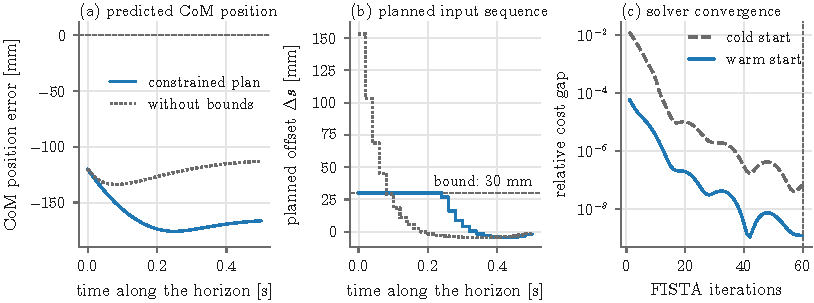
\includegraphics[width=\linewidth]{fig_mpc_plan.pdf}
  \caption{The horizontal MPC when the robot has been pushed backward. (a,b) The plan saturates the offset at its
  bound for half of the horizon and recovers more slowly than the unconstrained solution would. (c) Convergence of
  the solver; the controller stops at 60 iterations.}
  \label{fig:mpcplan}
\end{figure}

\subsection{Legs: virtual model control}

The MPC outputs a displacement and a force, and the legs must realise them. Virtual model
control~\cite{pratt2001} imagines a spring, a damper and a constant force acting between the hip and the wheel,
computes the force that these components would produce and maps it to the joints with the transpose of the leg
Jacobian. The law has the same form as \eqref{eq:legs}; the difference lies in what the components are asked to do.
Horizontally there is a spring: it holds the wheel at the distance $\delta$ behind the CoM, which is how the planned
offset is realised. Vertically there is \emph{no} spring, only a light damper, and each leg pushes with half of the
planned force $F_z$. The height is therefore not held by a stiffness: it is regulated by the MPC through the force.

Seen from the ground, each leg behaves as a force-controlled suspension rather than as a rigid strut. This is the
Cartesian impedance idea used in the course to make a legged robot compliant at its contacts, with the vertical
stiffness set to zero and the weight supplied as a feedforward. Its consequences on uneven ground are among the
clearest results of the next section.

% =====================================================================================================
\section{Benchmark and results}
\label{sec:results}

\subsection{Method}
\label{sec:benchmark}

The benchmark runs a catalogue of eleven scenarios with both controllers, one after the other, each from a clean
simulation: standing balance, an impulsive push, a constant force, a trapezoidal speed profile, a back-and-forth
motion, a change of height, a slow and a fast S-curve, and three stretches of uneven ground (speed bumps 2\,cm high, a
5\,\% ramp leading to a raised plateau, and a field of tiles of different heights that the two wheels cross on
different columns). In every run the robot is first held upright and then released, and time in the plots
is counted from the release. World, robot,
actuation and scenarios are identical, and every signal is recorded at 500\,Hz. The catalogue includes the tests with which the paper validates its controller in balance: change of height, recovery
from an impact and speed tracking. The
results below come from one complete execution of the suite.

\paragraph{Reconstructing the ZMP.} Since the simulator does not report contact forces, the centre of pressure
cannot be measured. The ZMP is therefore computed from its definition, summing the contribution of every link $i$ of
mass $m_i$ and position $(x_i,y_i,z_i)$, on flat ground:
\begin{equation}
  x_{zmp}=\frac{\sum_i m_i\big[(\ddot z_i+g)\,x_i-\ddot x_i\,z_i\big]-\sum_i\dot L_{y,i}}{\sum_i m_i(\ddot z_i+g)},
  \label{eq:zmp}
\end{equation}
and likewise for $y_{zmp}$, where $L_i$ is the angular momentum of the link about its own centre. Positions come
from the true pose of the torso and from the joint angles through the kinematics of the robot; accelerations are
obtained by fitting a parabola to a short window of samples, which avoids differentiating noise twice. Two
quantities are derived from it: the lateral position of the
ZMP as a fraction of the half-distance between the wheels, where 100\,\% means that the inner wheel is about to lift,
and the load on each wheel. In the direction of travel the ZMP must lie on the contact line, which provides a
check: on flat ground the reconstructed point stays within a millimetre of it.
Three cautions apply. First, the PID reads the pose of the torso from the
simulator, whereas the other controller estimates it; a perfect measurement favours the PID in smoothness. Second,
for the same reason the position that each controller measures is not the same signal. All the positions shown below
are therefore recomputed for both from the true pose, and so are the heights. This matters: on
straight paths the tracking error computed in this way is similar for the two laws, whereas the internal signals of
the controllers would suggest a clear advantage of the MPC, simply because its error is measured against its own odometry, which
can overestimate the distance travelled by up to about one per cent. Third, each scenario was run once, and small
differences fall within the variability from run to run. For these reasons only the differences that are large, and
that can be explained from the design of the controllers, are discussed.

\subsection{Disturbances: push and constant force}

\begin{figure}[t]
  \centering
  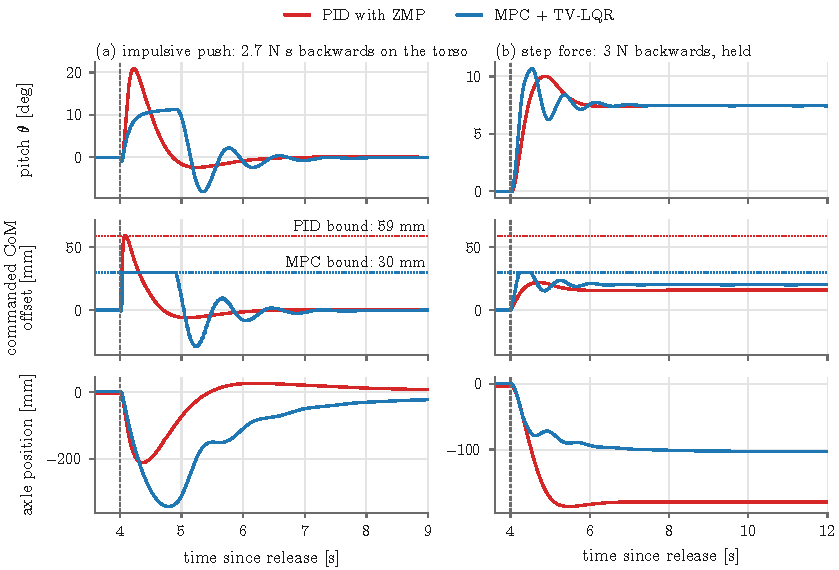
\includegraphics[width=\linewidth]{fig_disturbances.pdf}
  \caption{Response to disturbances applied to the torso four seconds after the release. Top: pitch of the
  equivalent pendulum. Middle: offset between centre of mass and contact commanded by each controller, with the
  bound that each imposes. Bottom: true position of the axle; the robot is asked to stay where it is.}
  \label{fig:disturb}
\end{figure}

The push is a short impulse that sends the torso backward at about 0.6\,m/s (Fig.~\ref{fig:disturb}a). The two
controllers react in opposite ways, and the middle panel shows why. The PID asks at once for the largest offset
that it allows, 6\,cm: the robot leans by about $20^\circ$, brakes hard, drifts by about 20\,cm, and its pitch is
back at rest in about two seconds with a single small overshoot. The MPC is bound to 3\,cm. It holds the offset on the bound for almost a
second, so the lean never exceeds about $11^\circ$, but the braking is gentler: the robot drifts by about 35\,cm and
needs a few oscillations to settle. Neither behaviour is right or wrong. They are the direct expression of the two
limits written in the controllers, $a_{max}$ in \eqref{eq:outer} and $\delta_{max}$ in \eqref{eq:mpc}, and they
show what a constraint in the plan achieves: the MPC keeps the posture within a prescribed envelope and
accepts a larger displacement in exchange. The linear model of Section~\ref{sec:authority}
predicts a peak of about $19^\circ$ for the PID: the simple model is a good guide to the simulated robot.

The constant force (Fig.~\ref{fig:disturb}b) asks a different question: what remains once the transient is over?
Both robots end up leaning into the force by the same angle, as statics demands. What differs is where they stand.
The PID stops about 18\,cm from the starting point, the MPC about 10\,cm. One might expect the integral term of the
PID to cancel the error. It does not, because the lean that balances this force requires an integral larger than its
anti-windup bound: the integral saturates, and the rest of the offset must come from the proportional term, that is
from a position error. Inserting the gains in~\eqref{eq:outer} gives 18\,cm, exactly what is measured.
The MPC has no integral action at all; its steady error is the point where the offset that its cost function is
willing to command for that position error equals the one needed to hold the force. A disturbance observer, such as
the momentum-based estimator presented in the course, would remove the error in both controllers and is the most
natural extension of this work.

\subsection{Tracking a planned motion}

\begin{figure}[t]
  \centering
  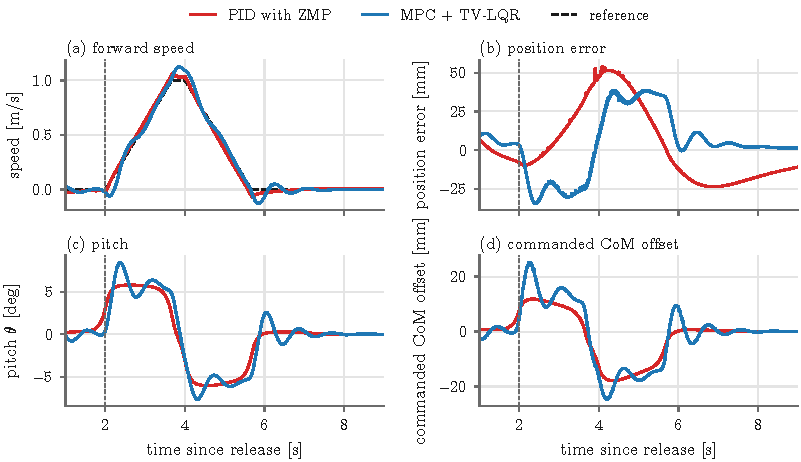
\includegraphics[width=\linewidth]{fig_tracking.pdf}
  \caption{Two metres forward with a trapezoidal speed profile (1\,m/s, 0.6\,m/s$^2$). The motion starts at the
  dashed line; the position error is computed from the true pose for both controllers.}
  \label{fig:tracking}
\end{figure}

In the trapezoid the robot must accelerate, cruise and brake (Fig.~\ref{fig:tracking}). The effect of the preview
is visible before the motion starts: when the reference begins to move, the PID is already leaning by a few degrees
(panel c). Its pitch then follows the shape that the plan requires---forward during the acceleration, level while
cruising, backward while braking---with hardly any overshoot, and it settles about a second after the stop. The
MPC does not know the acceleration step in advance in the same way: its horizon sees the reference half a second
ahead, but the cost only penalises the deviation of the CoM from it. Its pitch reaches the same plateau through
an overshoot and a few oscillations, and it needs several seconds to become quiet after braking. The oscillation
comes from the LQR following a reference that the MPC updates continuously, and it is the less satisfactory aspect
of this controller on RoTino. The position errors of the two laws are of the same size, a few centimetres at most
during the transients, although with different shapes. The back-and-forth scenario gives the same picture.

\subsection{Curved paths}

\begin{figure}[t]
  \centering
  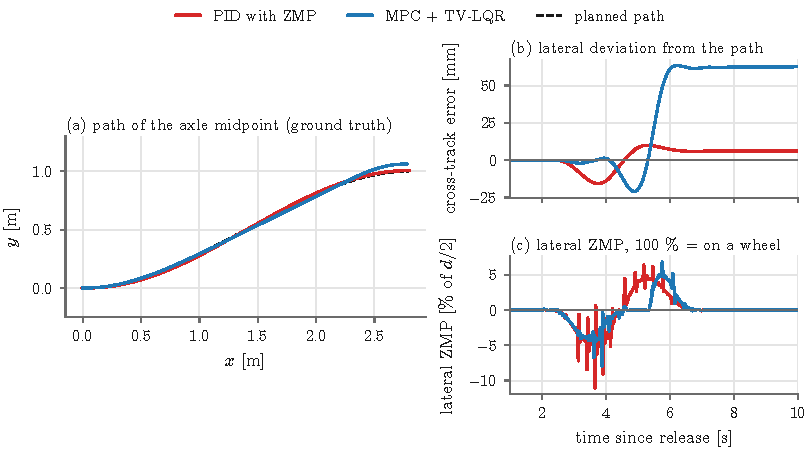
\includegraphics[width=\linewidth]{fig_scurve.pdf}
  \caption{The fast S-curve: three metres of path with a lateral displacement of one metre in five seconds.}
  \label{fig:scurve}
\end{figure}

On the S-curves the sagittal behaviour is that of the trapezoid, and the interest shifts to the plane
(Fig.~\ref{fig:scurve}). The PID stays within about a centimetre and a half of the path; the MPC deviates by up to
6\,cm and ends about 6\,cm to its side. The cause is not the estimator. Replaying the odometry on the recorded
encoder and gyroscope signals reproduces the true final position to within a few millimetres sideways, so the
controller knew where it was. The cause is the heading loop. To stay clear of the leg resonance, the LQR was given
a yaw stiffness that is half that of the PID, and with the friction of the wheels on the ground a soft loop leaves
a larger heading error; since the guidance \eqref{eq:guidance} fades out as the robot stops, what has not been
recovered by then remains. This is the price of the weighting choice of Section~\ref{sec:mpc}, and it suggests that
the resonance would be better treated at its source, by damping the yaw of the torso with the legs, than by slowing
the heading loop down.

The lateral ZMP gives the same message for both controllers (panel c). Even in the fast curve it moves by about a
tenth of the half-distance between the wheels: at these speeds the robot is far from tipping, and both wheels keep
most of their load. This is why the lateral compensation of the PID can remain switched off.

\subsection{Uneven ground}

\begin{figure}[t]
  \centering
  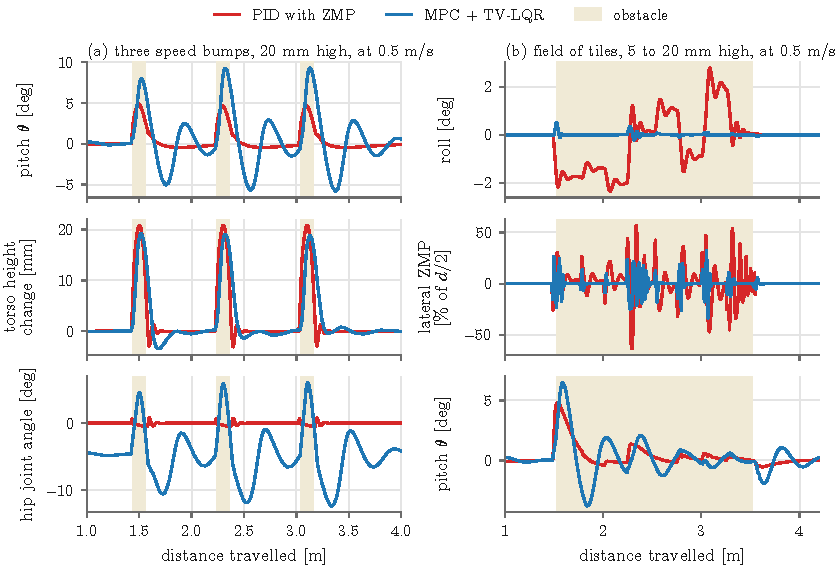
\includegraphics[width=\linewidth]{fig_terrain.pdf}
  \caption{Crossing the speed bumps and the field of tiles at 0.5\,m/s, plotted against the distance travelled.
  The change of height of the torso is computed from its true pose.}
  \label{fig:terrain}
\end{figure}

Neither controller knows anything about the ground: both assume that it is flat, and the platforms test how the
two structures absorb what they do not model (Fig.~\ref{fig:terrain}). On the ramp both simply climb and descend
with a pitch deviation of a degree or two; the more interesting cases are the other two.

\emph{Speed bumps.} A bump is a brief longitudinal disturbance on both wheels at once. The PID meets it with rigid
legs: the hip angle hardly moves, the pitch deviates by about $5^\circ$ and returns without oscillating. In the MPC
the disturbance propagates through the whole chain: the pitch error changes the planned offset, the legs swing by
almost $20^\circ$ to realise it, and the pitch reaches about $9^\circ$ and oscillates between one bump and the
next. In both cases the torso rises by the height of the bump. The height estimated by the MPC suggested otherwise,
because its estimator assumes flat ground and so does not see the bump at all; the comparison in the
figure uses the true pose for both.

\emph{Tiles.} Here the two wheels meet steps of different height, and the roles reverse. With the PID the torso
rolls by almost $3^\circ$: its legs are stiff position loops, so the difference of height between the two
wheels is transmitted to the body, the lateral ZMP is thrown towards one wheel by more than half of the available
margin, and the load on the other wheel drops to a third of its static value. With the MPC the roll stays near half
a degree, the excursion of the ZMP is roughly halved and the wheels remain better loaded. No part of that controller
controls the roll explicitly. The result is a property of virtual model control: each leg pushes with half of the
planned force whatever its length, so it lengthens or shortens to follow the step under its wheel. A choice made
for another reason---leaving the height to the MPC---turns out to give the robot a suspension.

\subsection{Overall picture}

Table~\ref{tab:summary} condenses the scenarios into the figures that characterise them, and the tally of the
benchmark over all its metrics is balanced: neither law dominates. What the results show is rather a pattern,
which follows from the structure of the two controllers.

\begin{table}[t]
  \centering\small
  \caption{Summary of the results (one run per scenario, rounded values).}
  \label{tab:summary}
  \begin{tabularx}{\linewidth}{@{}l>{\raggedright\arraybackslash}Xrr@{}}
    \toprule
    Scenario & Quantity & PID with ZMP & MPC + TV-LQR \\
    \midrule
    Standing balance & wheel torque needed to stand still & very low & three to four times higher \\
    Push & peak pitch & $21^\circ$ & $11^\circ$ \\
         & largest drift & 0.2\,m & 0.35\,m \\
    Constant force & steady displacement & 0.18\,m & 0.10\,m \\
    Trapezoid & peak pitch & $6^\circ$ & $8.5^\circ$ \\
              & time to settle after the stop & about 1\,s & more than 4\,s \\
    Height change & pitch deviation & \multicolumn{2}{c}{negligible for both} \\
    Fast S-curve & largest deviation from the path & 1.5\,cm & 6\,cm \\
                 & lateral ZMP, share of the margin used & \multicolumn{2}{c}{about one tenth for both} \\
    Speed bumps & peak pitch & $5^\circ$ & $9^\circ$ \\
    Ramp & peak pitch & \multicolumn{2}{c}{below $2^\circ$ for both} \\
    Tiles & peak roll & $3^\circ$ & $0.5^\circ$ \\
          & lateral ZMP, share of the margin used & about 60\,\% & about 35\,\% \\
    \bottomrule
  \end{tabularx}
\end{table}

The PID is at its best when the motion is known in advance. The preview lets it lean at the right moment, its
torques are small and smooth, and its pitch follows the plan without oscillating. Its limits are those of a
controller without constraints and with rigid legs: when it is surprised it reacts with all the lean it is allowed,
and uneven ground reaches the torso directly. It also relies, in this project, on a perfect measurement of the pose.

The MPC architecture is at its best where limits and contacts matter. The bound on the offset keeps the posture
within a known envelope under any disturbance, the force-controlled legs filter the ground, and all of this is
obtained using only the sensors of the robot. It pays with a more oscillatory pitch, with a soft heading loop and
with more parameters to tune; the computation, often seen as the cost of predictive control, is not an issue at
this scale.

A third lesson concerns the comparison itself. Several of the conclusions above differ from those that the raw
metrics of the benchmark suggested, because the two controllers measure position and height in different ways.
Comparing controllers fairly requires comparing the same physical quantities, and a simulator, which offers the true
state, makes this possible---provided that one remembers to use it.


\section{Conclusions}

A wheeled biped was modelled, simulated with torque control and balanced with two controllers built on the same
physical idea---the horizontal offset between the centre of mass and the contact sets the acceleration---and on
opposite philosophies. The cascaded PID treats that offset as the output of a capture-point loop and anticipates
planned motions with a preview. The architecture of Cui \emph{et al.}\ plans it with a constrained MPC and delegates
balance to a gain-scheduled LQR and compliance to the virtual model of the legs. On eleven scenarios neither is
uniformly better. The cascade is smoother and more accurate on planned motions; the predictive architecture keeps
the posture bounded under disturbances and behaves better on uneven ground. In almost every case the difference
could be traced to a specific line of the design: a bound, a weight, a stiffness.

The limits of the work indicate what should come next. The PID should be fed by the same estimator as the MPC, so
that the comparison is made on equal measurements, and each scenario should be repeated to quantify the variability.
A disturbance observer would remove the steady error under constant forces. The leg resonance that forced a soft
heading loop should be damped at its source. Finally, the wheels should be given a crowned profile, so that the
lateral ZMP can be controlled by leaning into curves and used as a constraint when turning at higher speed.

% =====================================================================================================
\begin{thebibliography}{99}\small
\setlength{\itemsep}{1pt}

\bibitem{cui2022} Z. Cui, Y. Xin, S. Liu, X. Rong, Y. Li, ``Modeling and control of a wheeled biped robot,''
\emph{Micromachines}, vol.~13, no.~5, 747, 2022.

\bibitem{klemm2019} V. Klemm \emph{et al.}, ``Ascento: a two-wheeled jumping robot,'' in \emph{Proc. IEEE Int. Conf.
on Robotics and Automation (ICRA)}, 2019, pp.~7515--7521.

\bibitem{spong1994} M. W. Spong, ``Partial feedback linearization of underactuated mechanical systems,'' in
\emph{Proc. IEEE/RSJ Int. Conf. on Intelligent Robots and Systems (IROS)}, 1994, pp.~314--321.

\bibitem{vukobratovic2004} M. Vukobratovi\'c, B. Borovac, ``Zero-moment point --- thirty five years of its life,''
\emph{Int. Journal of Humanoid Robotics}, vol.~1, no.~1, pp.~157--173, 2004.

\bibitem{kajita2003} S. Kajita, F. Kanehiro, K. Kaneko, K. Fujiwara, K. Harada, K. Yokoi, H. Hirukawa, ``Biped
walking pattern generation by using preview control of zero-moment point,'' in \emph{Proc. IEEE Int. Conf. on
Robotics and Automation (ICRA)}, 2003, pp.~1620--1626.

\bibitem{pratt2006} J. Pratt, J. Carff, S. Drakunov, A. Goswami, ``Capture point: a step toward humanoid push
recovery,'' in \emph{Proc. IEEE-RAS Int. Conf. on Humanoid Robots}, 2006, pp.~200--207.

\bibitem{englsberger2011} J. Englsberger, C. Ott, M. A. Roa, A. Albu-Sch\"affer, G. Hirzinger, ``Bipedal walking
control based on capture point dynamics,'' in \emph{Proc. IEEE/RSJ Int. Conf. on Intelligent Robots and Systems
(IROS)}, 2011, pp.~4420--4427.

\bibitem{brockett1983} R. W. Brockett, ``Asymptotic stability and feedback stabilization,'' in \emph{Differential
Geometric Control Theory}, Birkh\"auser, 1983, pp.~181--191.

\bibitem{pratt2001} J. Pratt, C.-M. Chew, A. Torres, P. Dilworth, G. Pratt, ``Virtual model control: an intuitive
approach for bipedal locomotion,'' \emph{Int. Journal of Robotics Research}, vol.~20, no.~2, pp.~129--143, 2001.

\bibitem{jerez2011} J. L. Jerez, E. C. Kerrigan, G. A. Constantinides, ``A condensed and sparse QP formulation for
predictive control,'' in \emph{Proc. IEEE Conf. on Decision and Control and European Control Conf.}, 2011,
pp.~5217--5222.

\bibitem{beck2009} A. Beck, M. Teboulle, ``A fast iterative shrinkage-thresholding algorithm for linear inverse
problems,'' \emph{SIAM Journal on Imaging Sciences}, vol.~2, no.~1, pp.~183--202, 2009.

\bibitem{fsr2026} F. Ruggiero, \emph{Field and Service Robotics}, lecture notes, University of Naples Federico II,
a.y.~2025/2026.

\end{thebibliography}

\end{document}
